\documentclass[xcolor=dvipsnames]{beamer} 
\usecolortheme[named=Blue]{structure} 
\usetheme[height=10.5mm]{Rochester} 
\setbeamertemplate{items}[ball] 
\setbeamertemplate{blocks}[rounded][shadow=true] 
\setbeamertemplate{navigation symbols}{} 
\usepackage{bm}
\usepackage{rotating}
\usepackage{graphicx}
\usepackage{multirow}
\usepackage{hyperref}
\usepackage{textcomp}
\usepackage{upquote}
\usepackage[absolute,overlay]{textpos}
\newenvironment{reference}[2]{%
  \begin{textblock*}{\textwidth}(#1,#2)
      \footnotesize\it\bgroup\color{red!50!black}}{\egroup\end{textblock*}}
%\graphicspath{ {/home/ben/PhD/Armidale_Updates/2014_03_14/Figures/} }
\begin{document}

\begin{frame} %1
% \frametitle{Addressing Common Challenges in Spatial Modeling of Ecologies and Environments}
%\begin{center}
\textbf{\huge Introduction to R}\\
Capstone Collaborative Exercise
%\end{center}

\begin{figure}
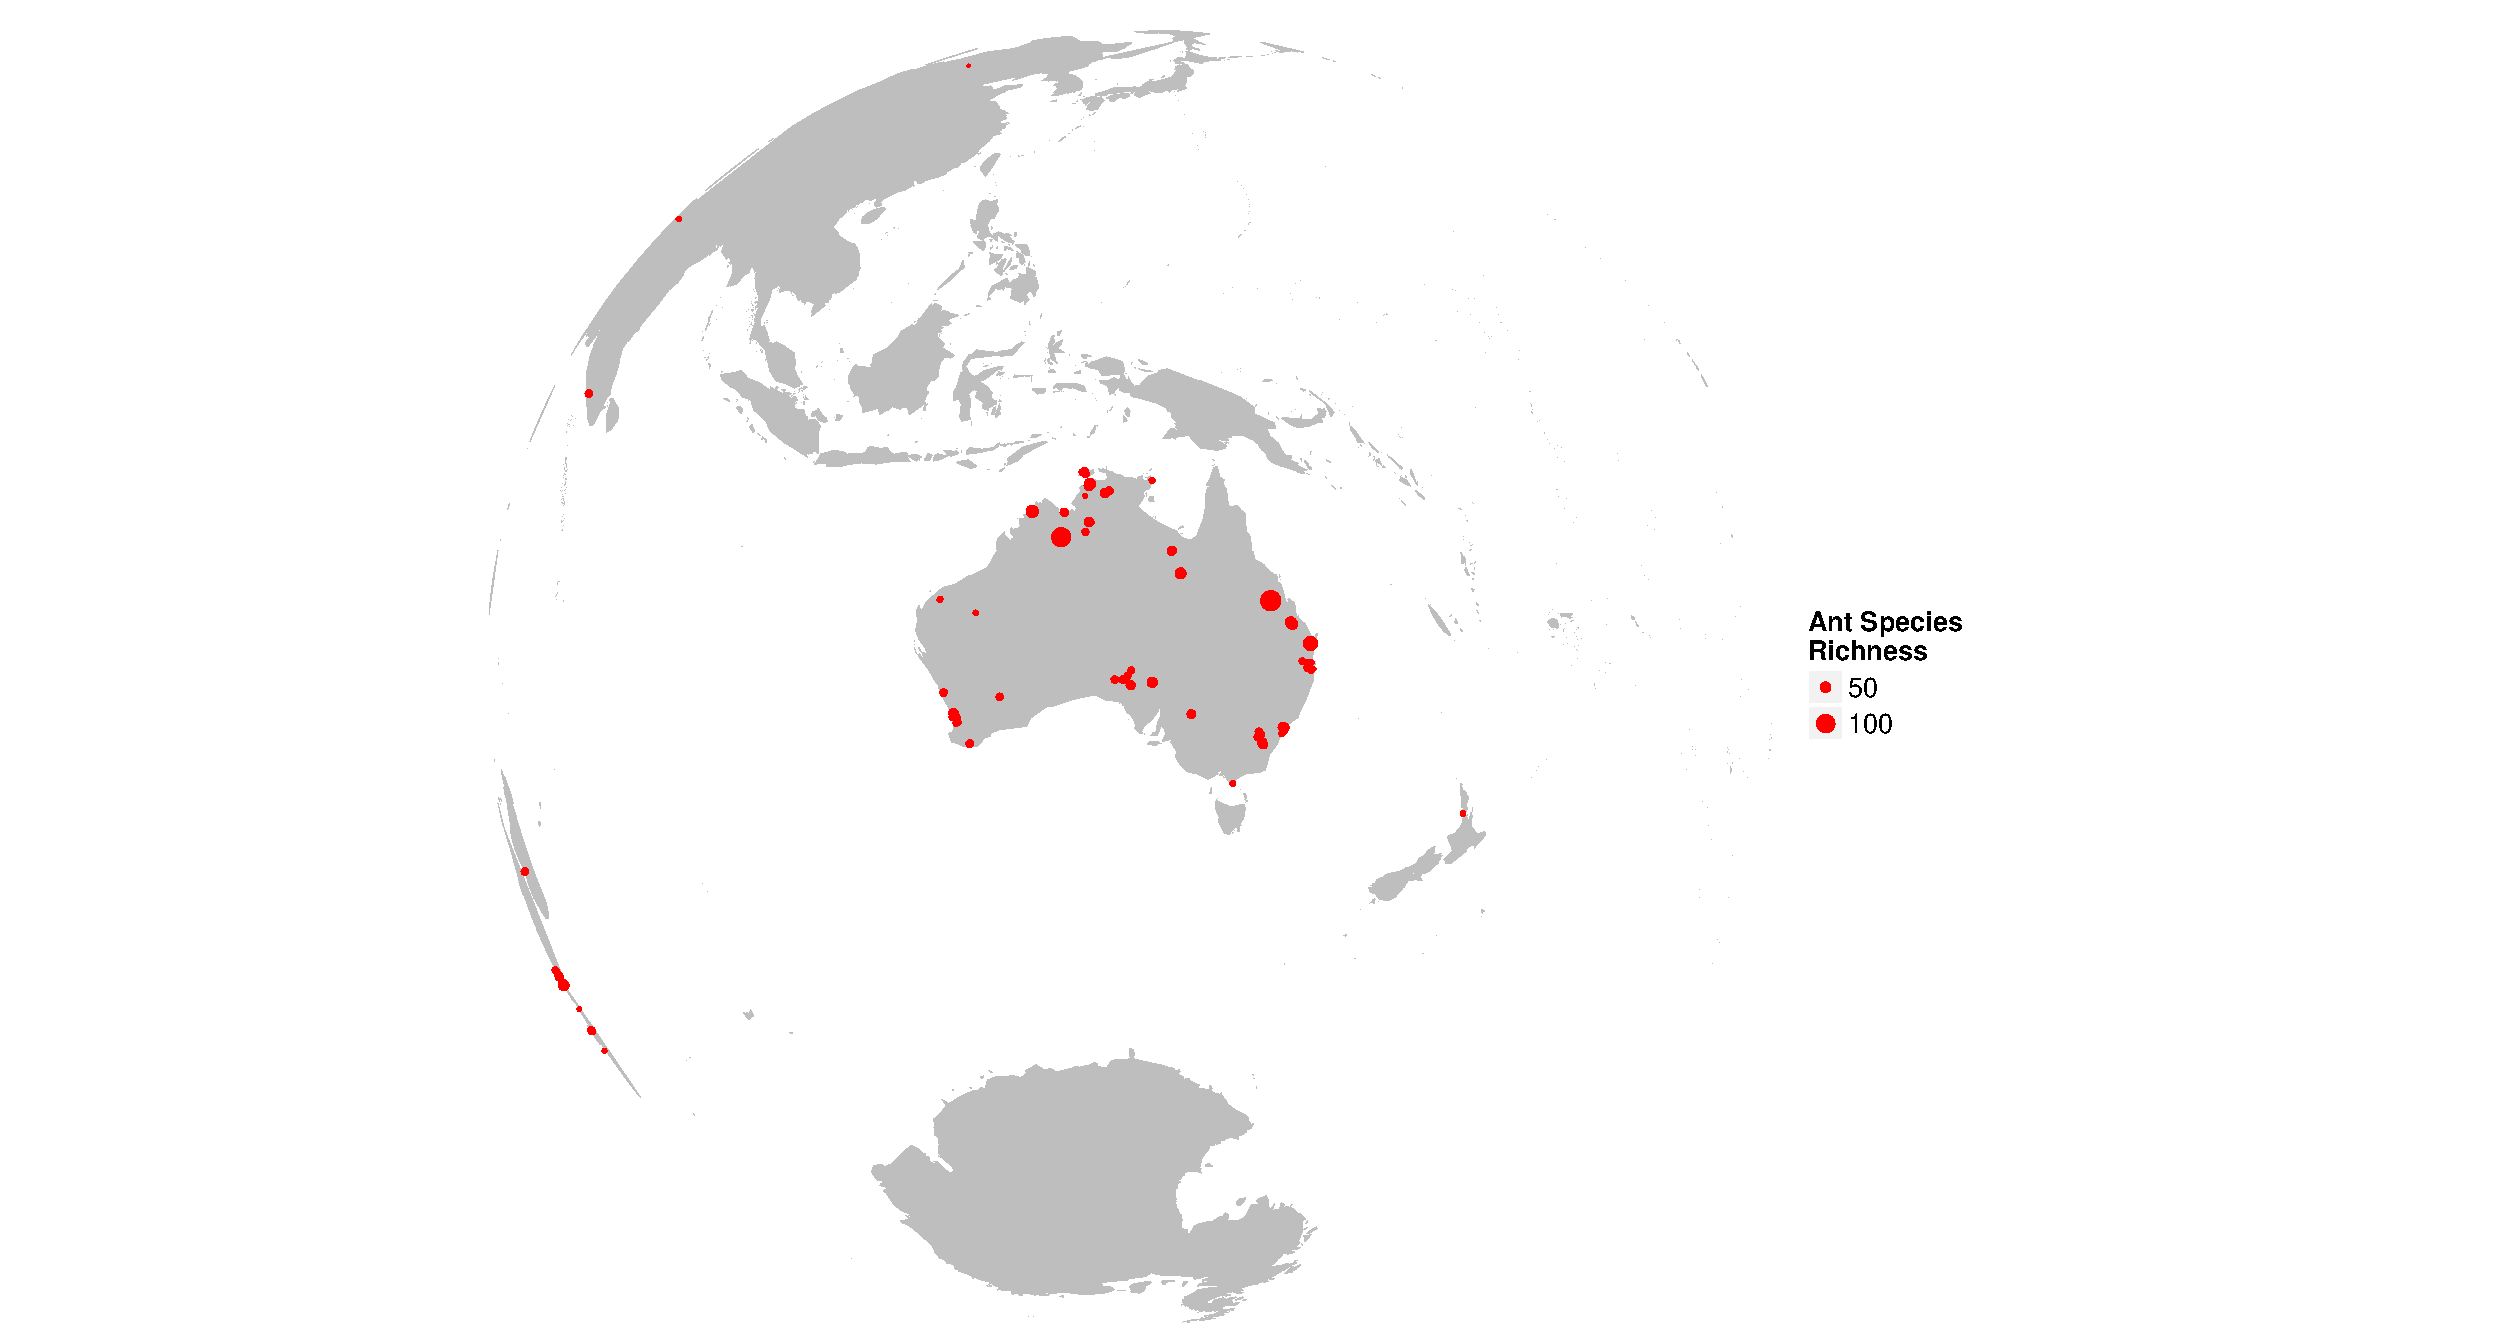
\includegraphics[width = 0.8\textwidth]{/home/ben/Intro_to_R/Capstone_Collaborative_Exercise/Capstone_Slides_Source/Images/Ant_Sp_Rich_Globe_Map.pdf}
\end{figure}
\small Ben R. Fitzpatrick\\
\tiny PhD Candidate, Statistical Science, Mathematical Sciences School, Queensland University of Technology
\newline
\begin{columns}
\begin{column}{3cm}
\tiny 0000-0003-1916-0939
\end{column}
\begin{column}{3cm}
\tiny github.com/brfitzpatrick/
\end{column}
\begin{column}{3cm}
\tiny @benrfitzpatrick
\end{column}
\end{columns}
\end{frame}

\begin{frame}
\frametitle{Modelling Ant Species Richness with Climate \& Habitat}
\framesubtitle{Opportunity to practise skills learned in this course}

\begin{figure}
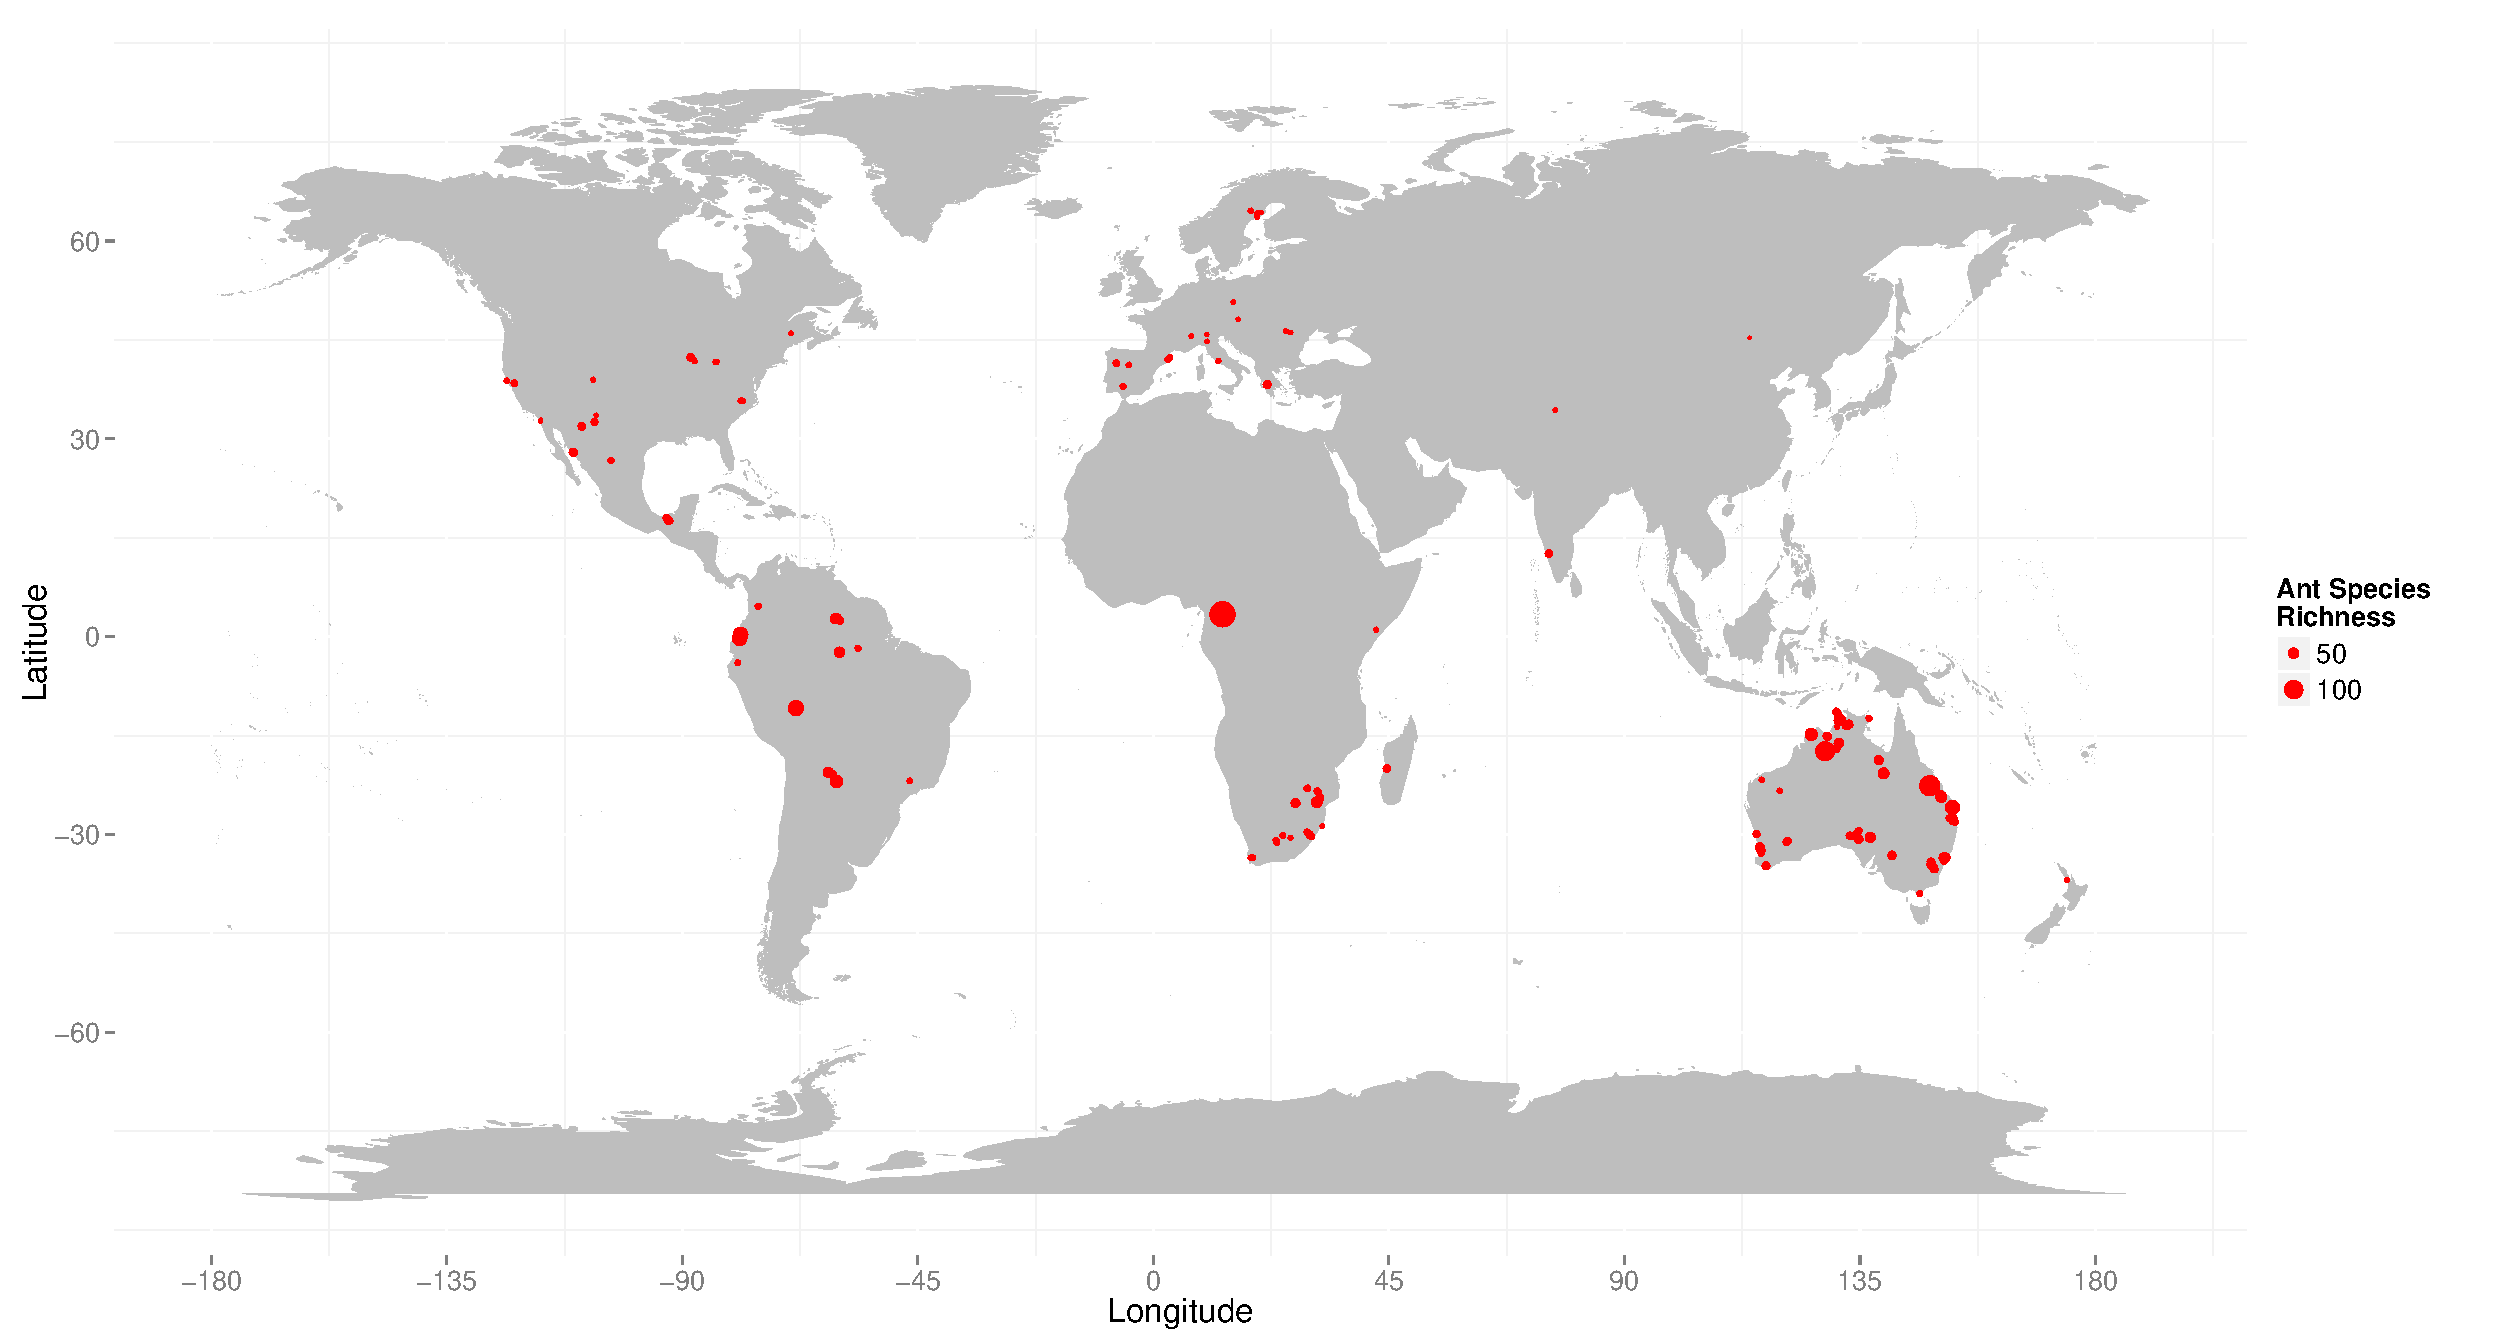
\includegraphics[width = \textwidth]{/home/ben/Intro_to_R/Capstone_Collaborative_Exercise/Capstone_Slides_Source/Images/Ant_Sp_Rich_Map.pdf}
\end{figure}

\end{frame}

\begin{frame}
\frametitle{Goals}
Workflow:
\begin{enumerate}
\item Summarise \& Visualise the Data
\item Formulate Analysis Questions
\item Choose Model
\item Fit Model
\item Produce and Interpret Model Diagnostics
\item Produce \& Interpret Model Summary Statistics
\item Predict from Model and Quantify Uncertainty Associated with these Predictions
\item Reflect \& Revise Analysis Questions
\item Potentially, Repeat...
\end{enumerate}
\end{frame}

\begin{frame}
\frametitle{Meet the Data}
\framesubtitle{Ant Species Richness at Sites around the Globe}
This exercise uses some publicly available data from the Dryad Repository. Please download a copy of `Data appendix.xlsx' from:
\newline
\newline
\url{http://dx.doi.org/10.5061/dryad.r36n0}
\newline
\newline
These data were published as part of:
\newline
\newline
\small Gibb H, Sanders NJ, Dunn RR, Watson S, Photakis M, Abril S, Andersen AN, Angulo E, Armbrecht I, Arnan X, Baccaro FB, Bishop TR, Boulay R, Castracani C, Del Toro I, Delsinne T, Diaz M, Donoso DA, Enríquez ML, Fayle TM, Feener DH, Fitzpatrick MC, Gómez C, Grasso DA, Groc S, Heterick B, Hoffmann BD, Lach L, Lattke J, Leponce M, Lessard J, Longino J, Lucky A, Majer J, Menke SB, Mezger D, Mori A, Munyai TC, Paknia O, Pearce-Duvet J, Pfeiffer M, Philpott SM, de Souza JLP, Tista M, Vasconcelos HL, Vonshak M, Parr CL (2015) \textit{Climate mediates the effects of disturbance on ant assemblage structure}. \textbf{Proceedings of the Royal Society B} 282(1808).
\end{frame}

\begin{frame}
For today let's focus on Species Richness as a response variable and ignore the hierarchy in the data (as coded by the `cluster' variable)
\newline
\newline
If we do this we can consider a preliminary analysis with Multiple Linear Regression or Generalized Linear Models.
\newline
\newline
This is OK for practise but if we were seriously attempting this analysis for publication etc. we'd need to consider incorporating random effects for cluster or modelling the cluster means...if you feel confident to try one of these options please do...
\begin{table}[ht]
\centering
\tiny
\begin{tabular}{ccccccccccc}
  \hline
Lat. & Long. & Mean & Total & Temp. & Disturb. & Hemi & Cont. & Pitfall & Trans. & Species  \\
 &  & annual & annual & range &  &  &  & days & length & richness  \\
 &  & temp. & precip. &  &  &  &  &  &  &  \\
  \hline
 -22.5 & 148.3 & 21.90 & 615 & 25.40 & Undist. & South & Oceania & 450 & 40 &  75 \\ 
 -22.5 & 148.3 & 21.90 & 615 & 25.40 & Dist. & South & Oceania & 300 & 40 &  55  \\ 
 -22.5 & 148.3 & 21.90 & 615 & 25.40 & Dist. & South & Oceania & 300 & 40 &  50  \\ 
 -22.5 & 148.3 & 21.90 & 615 & 25.40 & Dist. & South & Oceania & 300 & 40 &  38  \\ 
 -22.5 & 148.3 & 21.90 & 615 & 25.40 & Dist. & South & Oceania & 300 & 40 &  46  \\ 
 -22.5 & 148.3 & 21.90 & 615 & 25.40 & Undist. & South & Oceania & 450 & 40 &  87 \\ 
   \hline
\end{tabular}
\end{table}
\end{frame}

\begin{frame}
\frametitle{Some Ideas...}

Article title:\\
\textit{Climate mediates the effects of disturbance on ant assemblage structure}.\\
suggests interaction terms may be important here \begin{itemize}
 \item as variables are on different scales it will be advisable to recenter and rescale them all to a common mean and magnitude (0, 1) is the traditional choice
\newline
\end{itemize}
Species Richness is not continuous (it's non-negative integers) so: \begin{itemize}
\item a Generalized Linear Model would be a good idea
\item however there is quite a range in the response so Multiple Linear Regression will be OK here for our purposes if you'd like to keep it simple
\newline
\end{itemize} 
\end{frame}


\begin{frame}
\frametitle{Options for Extension}

\begin{block}{Model for Probability of Interspecific Encounter (PIE)}
PIE is bounded between 0 and 1 (it's a probability!) \begin{itemize}
\item so a logit transformation would be necessary in order to model it with a linear model...\end{itemize}
\end{block}

\begin{block}{Accounting for Hierarchy in Data}
`Because sites were spatially clustered, we used mixed-effects models, with clusters of sites separated by no more than 100 km from each other represented by a single random effect to control for potential autocorrelation between localized sites' - Gib et al.
\begin{itemize}
\item Simpler option: calculate cluster means and model those...
\item Better option: use linear mixed effects models as Git et al. did  \end{itemize}
\end{block}

\end{frame}


\begin{frame} 
\frametitle{Over to you...}
\begin{itemize}
\item Please form small groups
\newline
\item Together I'd like you to collaboratively plan and conduct an exploratory analysis of these data
\newline
\item Please write neat, well annotated code and share this code with your group members via a GitHub repository
\newline
\item prior to the end of the course each group will present their methods and code along with their results and interpretation 
\end{itemize}
\end{frame}


\begin{frame}
\frametitle{Some possible Questions}
\begin{enumerate}
\item Is climate a useful predictor of the variation in ant species richness?
\item Is habitat disturbance a useful predictor of the variation in ant species richness?
\item Does habitat disturbance influence the nature of the correlation between climate and ant species richness?
\item Are there non-linear correlations between ant species richness and the continuous covariates?
\item Does habitat disturbance influence the nature of the correlation between climate and ant species richness after all other covariate effects have been accounted for?
\item Do models that incorporate non-linear effects and interactions out perform model that include only linear effects?
\item Can you use a variable selection technique to build a parsimonious model from the full set of linear, non-linear and interaction terms for the covariates included in these data?
\end{enumerate}
\end{frame}

\begin{frame}[fragile]
\frametitle{A quick note on reading the data into R}
The data file available on the Dryad Repository, `Data appendix.xlsx', has two columns we don't really need.\newline
\newline
When using your Spread Sheet program (Excel, Calc, etc.) to convert the .xlsx file to a .csv feel please delete the columns:
\begin{verbatim} `Locality_ID' \end{verbatim} and
\begin{verbatim} `Source'      \end{verbatim}
 for a less text heavy dataframe to read into R.
\end{frame}

\begin{frame}[fragile]
\frametitle{Solutions}

A code file containing annotated code to complete a multiple linear regression based analysis of the potential relationships between ant species richness, climate and habitat distrubance is available at:
\newline
\newline
\url{https://github.com/brfitzpatrick/Intro_to_R/blob/master/Collaborative_Exercise_Solutions.R}

\end{frame}

\end{document}